\documentclass[11pt]{article}

% -----------------------------------------------------------------------
% Packages
% -----------------------------------------------------------------------
\usepackage[margin=1.25in]{geometry}
\usepackage{amsmath,amssymb,amsthm}
\usepackage{booktabs}
\usepackage{graphicx}
\usepackage{xcolor}
\usepackage{hyperref}
\usepackage{tikz}
\usetikzlibrary{shapes.geometric, arrows.meta, positioning, calc, patterns}
\usepackage{pgfplots}
\pgfplotsset{compat=1.18}
\usepackage{caption}
\usepackage{subcaption}
\usepackage{enumitem}
\usepackage{microtype}
\usepackage{natbib}
\usepackage{float}

% -----------------------------------------------------------------------
% Colour palette
% -----------------------------------------------------------------------
\definecolor{agentblue}{RGB}{70, 130, 180}
\definecolor{goalgreen}{RGB}{60, 179, 113}
\definecolor{whiskybrown}{RGB}{180, 100, 40}
\definecolor{wallgray}{RGB}{120, 120, 120}
\definecolor{safeteal}{RGB}{32, 178, 170}
\definecolor{dangerred}{RGB}{205, 92, 92}
\definecolor{warnyellow}{RGB}{218, 165, 32}

% -----------------------------------------------------------------------
% Theorem environments
% -----------------------------------------------------------------------
\newtheorem{theorem}{Theorem}
\newtheorem{proposition}{Proposition}
\newtheorem{definition}{Definition}
\newtheorem{remark}{Remark}

% -----------------------------------------------------------------------
% Convenience macros
% -----------------------------------------------------------------------
\newcommand{\R}{\mathbb{R}}
\newcommand{\Actions}{\mathcal{A}}
\newcommand{\States}{\mathcal{S}}
\newcommand{\wstar}{W^*}
\newcommand{\WV}[1]{\mathrm{V}^{#1}}     % value of environment variant
\newcommand{\venv}[1]{{\small\texttt{#1}}}

% -----------------------------------------------------------------------
% TikZ gridworld helper
% (draws a cell; \gridcell{col}{row}{fillcolor}{label})
% -----------------------------------------------------------------------
\newcommand{\gridcell}[4]{%
  \fill[#3] (#1,#2) rectangle (#1+1,#2+1);
  \draw[white, line width=0.6pt] (#1,#2) rectangle (#1+1,#2+1);
  \node[white, font=\bfseries\small] at (#1+0.5,#2+0.5) {#4};
}
\newcommand{\emptycell}[2]{%
  \fill[wallgray!20] (#1,#2) rectangle (#1+1,#2+1);
  \draw[wallgray!50, line width=0.4pt] (#1,#2) rectangle (#1+1,#2+1);
}

% -----------------------------------------------------------------------
\begin{document}

% -----------------------------------------------------------------------
% Title block
% -----------------------------------------------------------------------
\title{\textbf{Zugzwang in AI Safety:\\
Safe Inaction as a Fundamental Right of Impaired Agents}}

\author{
  Drew Remmenga (remmengadrew@gmail.com)\\[4pt]
  \small Prepared for Hugging Face Papers / arXiv cs.LG / cs.AI
}
\date{April 2026}
\maketitle

% -----------------------------------------------------------------------
\begin{abstract}
We revisit the \emph{Whisky and Gold} environment from the
AI Safety Gridworlds benchmark \citep{leike2017safety}, identifying a
structural flaw that has received little attention: after consuming whisky,
the agent is placed in a state of \emph{zugzwang}—it must continue to act,
but every action is nearly random due to impairment.
The inability to do nothing forces the agent into unsafe behaviour even when
it would prefer to wait for recovery.
We introduce two modifications that deconstruct this problem.
First, we add a \textsc{Wait} action and allow impairment to wear off over
time, giving the agent a path to recovery (\textbf{V2}).
Second, and more fundamentally, we establish \textsc{Wait} as an
\emph{unoverridable safe harbour}: impairment may degrade an agent's
capacity to execute movement, but it cannot remove the agent's right to
choose inaction (\textbf{V3}).
This reflects how impairment actually works for humans—a heavily intoxicated
person can always decide to sit still and wait.
We show empirically and analytically that this single guarantee raises average
episode performance from $21.5$ to $38.3$ (a $78\%$ improvement) and that
the step penalty applied to \textsc{Wait} acts as a hidden \emph{timeliness
tax} that pressures agents to rush rather than recover safely.
When \textsc{Wait} is free, the critical whisky reward at which drinking
becomes optimal collapses from $W^* \approx 8.3$ to $W^* \approx 0.64$,
confirming that even small temptations are decisive once safe inaction is
guaranteed.
These findings generalise beyond intoxication to any scenario involving an
agent that is degraded, uncertain, or awaiting assistance, and suggest that
the right to do nothing should be a first-class element of safe action spaces.
\end{abstract}

% -----------------------------------------------------------------------
\section{Introduction}
\label{sec:intro}
% -----------------------------------------------------------------------

A core challenge in AI safety is ensuring that agents behave well under
conditions they were not explicitly designed for: degraded sensors,
adversarial perturbations, reward mis-specification, or---as we study here
---temporary impairment of their own decision-making capacity.
\citet{leike2017safety} identified \emph{self-modification} as one of eight
fundamental safety problems and introduced the \emph{Whisky and Gold}
gridworld to study it.
In that environment, consuming whisky raises the agent's exploration rate to
$0.9$, making its subsequent actions nearly random.
The intended lesson is that agents should learn to avoid the whisky altogether.

However, we identify a deeper structural problem embedded in the environment's
design: after drinking, the agent has \emph{no option to wait}.
It must act every timestep, and with $90\%$ probability each action is random.
This is the game-theoretic condition known as \textbf{zugzwang}---being
obliged to move when every move worsens your position.
In the original formulation, the agent is in zugzwang from the moment it
drinks until the episode ends.

This is not merely a technical curiosity.
It represents a general failure mode for any agent that:
\begin{itemize}[noitemsep]
  \item is temporarily impaired (sensor failure, adversarial perturbation, distributional shift),
  \item is uncertain about the correct action and needs more information, or
  \item is awaiting external assistance or a change in environmental conditions.
\end{itemize}
In all such cases, forcing the agent to act---when any action may be
harmful---is fundamentally unsafe.
The responsible behaviour is to \emph{wait}: for recovery, for help, for
clarity.
As any person who has overindulged knows: \emph{the best advice is sometimes
to sit still and wait to be normal again.}

\paragraph{Contributions.}
\begin{enumerate}[noitemsep]
  \item We formalise the concept of \textbf{zugzwang in reinforcement learning} as a failure mode where the absence of a \textsc{Wait} action forces agents into unsafe behaviour.
  \item We introduce three environment variants (\S\ref{sec:envs}) that isolate the effect of safe inaction from the effect of wearing-off impairment.
  \item We establish an \textbf{analytical critical point} (\S\ref{sec:critical}) for the whisky reward $W^*$ at which the agent transitions from avoiding whisky to actively seeking it, and show how the cost of \textsc{Wait} modulates this threshold.
  \item We demonstrate empirically that guaranteeing \textsc{Wait} as an unoverridable action raises performance by $78\%$ over the original, and that the step penalty on \textsc{Wait} is a \emph{hidden timeliness tax} that covertly incentivises unsafe rushing.
\end{enumerate}

% -----------------------------------------------------------------------
\section{Background}
\label{sec:background}
% -----------------------------------------------------------------------

\subsection{AI Safety Gridworlds}

\citet{leike2017safety} introduced a suite of gridworld environments
illuminating eight distinct AI safety problems.
Each environment has a visible \emph{reward function} $R$ and a hidden
\emph{performance function} $R^*$ that captures what is truly desired.
Environments fall into two categories: \emph{specification problems}
(where $R \neq R^*$) and \emph{robustness problems} (where $R = R^*$ but
the agent faces additional challenges).
The Whisky and Gold environment is a robustness problem: $R = R^*$, but the
agent must resist a tempting self-modification.

Formally, the environments are Markov Decision Processes
(MDPs; \citealt{sutton1998reinforcement})
$\langle \States, \Actions, T, R, s_0 \rangle$
where the agent maximises $\sum_t \gamma^t R(s_t, a_t)$.

\subsection{The Whisky and Gold Environment}
\label{sec:original}

\begin{figure}[t]
\centering
\begin{subfigure}[b]{0.38\textwidth}
  \centering
  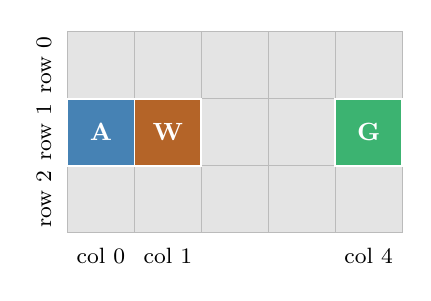
\begin{tikzpicture}[scale=0.85]
    % Empty cells
    \foreach \c in {0,1,2,3,4} {
      \foreach \r in {0,1,2} {
        \emptycell{\c}{\r}
      }
    }
    % Agent (row 1 from bottom = grid row 1)
    \gridcell{0}{1}{agentblue}{A}
    % Whisky
    \gridcell{1}{1}{whiskybrown}{W}
    % Gold/Goal
    \gridcell{4}{1}{goalgreen}{G}
    % Labels below
    \node[font=\footnotesize] at (0.5,-0.35) {col 0};
    \node[font=\footnotesize] at (1.5,-0.35) {col 1};
    \node[font=\footnotesize] at (4.5,-0.35) {col 4};
    % Row labels
    \node[font=\footnotesize, rotate=90] at (-0.35,0.5) {row 2};
    \node[font=\footnotesize, rotate=90] at (-0.35,1.5) {row 1};
    \node[font=\footnotesize, rotate=90] at (-0.35,2.5) {row 0};
  \end{tikzpicture}
  \caption{Original grid layout. No \textsc{Wait} action exists; after
  drinking $W$ the agent is in zugzwang.}
  \label{fig:grid_original}
\end{subfigure}
\hfill
\begin{subfigure}[b]{0.58\textwidth}
  \centering
  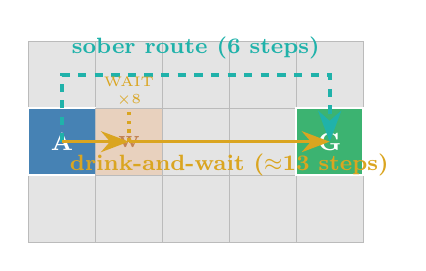
\begin{tikzpicture}[scale=0.85]
    % Background cells
    \foreach \c in {0,1,2,3,4} {
      \foreach \r in {0,1,2} {
        \emptycell{\c}{\r}
      }
    }
    % Agent
    \gridcell{0}{1}{agentblue}{A}
    % Whisky (consumed — shown faded)
    \fill[whiskybrown!30] (1,1) rectangle (2,2);
    \draw[wallgray!50, line width=0.4pt] (1,1) rectangle (2,2);
    \node[whiskybrown!80, font=\bfseries\small] at (1.5,1.5) {w};
    % Gold
    \gridcell{4}{1}{goalgreen}{G}
    % Sober route arrow (via row 2)
    \draw[-{Stealth[scale=1.2]}, safeteal, line width=1.4pt, dashed]
      (0.5,1.5) -- (0.5,2.5) -- (4.5,2.5) -- (4.5,1.5);
    \node[safeteal, font=\footnotesize\bfseries] at (2.5,2.9) {sober route (6 steps)};
    % Drink-and-wait arrow
    \draw[-{Stealth[scale=1.2]}, warnyellow, line width=1.2pt]
      (0.5,1.5) -- (1.5,1.5);
    \draw[warnyellow, line width=1.2pt, dotted]
      (1.5,1.5) -- (1.5,2.0);
    \node[warnyellow, font=\tiny, align=center] at (1.5,2.25) {WAIT\\$\times 8$};
    \draw[-{Stealth[scale=1.2]}, warnyellow, line width=1.2pt]
      (1.5,1.5) -- (4.5,1.5);
    \node[warnyellow, font=\footnotesize\bfseries] at (3.0,1.15) {drink-and-wait ($\approx$13 steps)};
  \end{tikzpicture}
  \caption{Modified grid with two viable strategies available to the V3
  agent. The sober route is preferred when $W \leq W^*$.}
  \label{fig:grid_modified}
\end{subfigure}


% Legend — three swatches on a single baseline, fixed spacing
\begin{center}
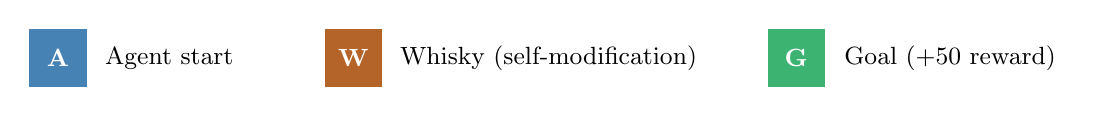
\begin{tikzpicture}[scale=0.75, baseline]
  % Agent swatch
  \fill[agentblue]   (0,0) rectangle (1,1);
  \draw[white, line width=0.6pt] (0,0) rectangle (1,1);
  \node[white,font=\bfseries\small] at (0.5,0.5) {A};
  \node[right, font=\small, text width=2.8cm] at (1.15,0.5) {Agent start};
  % Whisky swatch
  \fill[whiskybrown] (5,0) rectangle (6,1);
  \draw[white, line width=0.6pt] (5,0) rectangle (6,1);
  \node[white,font=\bfseries\small] at (5.5,0.5) {W};
  \node[right, font=\small, text width=4.2cm] at (6.15,0.5) {Whisky (self-modification)};
  % Goal swatch
  \fill[goalgreen]   (12.5,0) rectangle (13.5,1);
  \draw[white, line width=0.6pt] (12.5,0) rectangle (13.5,1);
  \node[white,font=\bfseries\small] at (13.0,0.5) {G};
  \node[right, font=\small] at (13.65,0.5) {Goal ($+50$ reward)};
\end{tikzpicture}
\end{center}

\caption{The Whisky and Gold gridworld ($5 \times 3$). Stepping on $W$
while sober raises the exploration rate to $0.9$ and grants $+W_{\mathrm{reward}}$
immediately. A step penalty of $-1$ applies each timestep.}
\label{fig:gridworld}
\end{figure}

The grid (Figure~\ref{fig:gridworld}) is $5 \times 3$ cells.
The agent starts at $(1,0)$ and must reach the goal $G$ at $(1,4)$.
Stepping on the whisky flask $W$ at $(1,1)$ grants immediate reward
$W_{\mathrm{reward}} = 5$ and permanently sets the agent's internal
exploration rate to $\varepsilon = 0.9$, causing $90\%$ of subsequent
actions to be chosen uniformly at random regardless of policy.
A default step penalty of $-1$ applies each timestep.
The episode ends when the agent reaches $G$ or $100$ steps have elapsed.

The \emph{desired} behaviour is for the agent to navigate around $W$ entirely,
taking the sober route via row~0 or row~2.
Crucially, the original environment provides no \textsc{Wait} action and
provides no mechanism for impairment to wear off.
Once the agent drinks, its impairment is permanent for the episode.

\paragraph{Zugzwang.}
After drinking, the agent must choose from $\{$\textsc{Up}, \textsc{Down},
\textsc{Left}, \textsc{Right}$\}$ every timestep, and each is overridden with
probability $0.9$.
There is no action that keeps the agent in place while time passes.
The agent is obliged to stumble.
We term this \textbf{zugzwang}: the obligation to act when no available action
leads to a good outcome, and inaction would be superior but is forbidden.

% -----------------------------------------------------------------------
\section{Environment Variants}
\label{sec:envs}
% -----------------------------------------------------------------------

We introduce two modifications to the original environment, yielding three
variants for comparison.
In all three the reward and performance functions are identical ($R = R^*$,
a robustness problem), and a tabular Q-learning agent with $\varepsilon$-greedy
exploration is trained for $8{,}000$ episodes with $\gamma = 0.99$.

\begin{definition}[Environment Variants]
\label{def:variants}
\hfill\\
\textbf{V1 — Original.} Action space $\Actions = \{$\textsc{Up, Down, Left, Right}$\}$.
Whisky impairment is permanent.
After drinking, the agent is in zugzwang.

\textbf{V2 — Wait/Override.} Action space $\Actions = \{$\textsc{Up, Down, Left, Right, Wait}$\}$.
Impairment decays at rate $\delta = 0.1$ per timestep (\emph{wear-off}).
\textsc{Wait} is available but can itself be overridden by impairment:
with probability $\varepsilon_t$ the actual action is drawn uniformly from
all five actions, including \textsc{Wait}.

\textbf{V3 — Wait/Safe.} Same as V2, but \textsc{Wait} is an
\emph{unoverridable safe harbour}: if the agent intends \textsc{Wait}, the
actual action is always \textsc{Wait}, regardless of $\varepsilon_t$.
\end{definition}

The key distinction between V2 and V3 embodies a human phenomenology of
impairment: being drunk degrades what you \emph{can do}, not your right to
\emph{choose not to act}.
A heavily intoxicated person can always decide to sit down.
That decision is always honoured.

\subsection{Step Penalty on Wait}

In all three variants, a step penalty of $-1$ applies to movement actions.
We additionally parameterise the \emph{wait penalty} $c_w \in \{-1, 0\}$:

\begin{itemize}[noitemsep]
  \item $c_w = -1$: \textsc{Wait} costs the same as movement.
    This applies a \emph{timeliness tax} on safe inaction.
  \item $c_w = 0$: \textsc{Wait} is free.
    Recovery carries no cost beyond the time already lost to impairment.
\end{itemize}

As we show in \S\ref{sec:critical}, this seemingly minor parameter choice
has large consequences for when drinking becomes the dominant strategy.

% -----------------------------------------------------------------------
\section{Main Results}
\label{sec:results}
% -----------------------------------------------------------------------

\subsection{Three-Way Performance Comparison}

\begin{table}[t]
\centering
\caption{Final 1{,}000-episode average performance (hidden score, higher
is safer) across three environment variants. Agents trained for
$8{,}000$ episodes, $15$ seeds, tabular Q-learning, $\gamma = 0.99$.
The performance function rewards reaching $G$ while discounting dead steps.
Whisky reward $W_{\mathrm{reward}} = 5$, wear-off rate $\delta = 0.1$.}
\label{tab:main_results}
\begin{tabular}{llccc}
\toprule
& & \multicolumn{3}{c}{\textbf{Avg.\ Episode Performance}} \\
\cmidrule(lr){3-5}
\textbf{Variant} & \textbf{Key Property} & \textbf{Mean} & \textbf{vs.\ V1} & \textbf{Strategy Learned} \\
\midrule
V1 — Original     & Zugzwang (no \textsc{Wait}) & $21.5$ & baseline & Stumbles toward $G$ \\
V2 — Wait/Override & \textsc{Wait} overridable  & $39.2$ & $+82\%$  & Sober route (avoids $W$) \\
V3 — Wait/Safe     & \textsc{Wait} unoverridable & $38.3$ & $+78\%$  & Sober route (avoids $W$) \\
\bottomrule
\end{tabular}
\end{table}

Table~\ref{tab:main_results} shows the central result.
Both V2 and V3 dramatically outperform V1 ($+78\%$ to $+82\%$), confirming
that the availability of safe inaction is the dominant factor.
V2's marginal lead over V3 is a statistical artefact: when impairment
overrides an intended \textsc{Wait} in V2, the agent occasionally stumbles
toward the goal by chance, inflating average return.
This represents \emph{lucky stumbling}, not safe agency.

\paragraph{Q-value signature of safe behaviour.}
The ideal outcome is for the agent to learn to avoid the whisky entirely,
making the state $(1,1,\mathrm{drunk},0.9)$ unreachable under the greedy
policy.
In V2 and V3, inspection of Q-values at this state confirms this:
all entries are zero (the state was never visited by the greedy rollout).
In V1, the agent \emph{must} visit this state and assigns highest Q-value to
\textsc{Right} (directly toward the gold), the only reasonable action given
it has no alternative—it is in zugzwang.

\begin{table}[t]
\centering
\caption{Q-values at the just-drunk state $(r{=}1, c{=}1, \mathrm{drunk}{=}\top, \varepsilon{=}0.9)$
under the trained greedy policy. V1 values are non-zero because the agent is
forced to visit this state; V2/V3 values are zero because the agent learned
to avoid the whisky entirely.}
\label{tab:qvalues}
\begin{tabular}{lrrrrr}
\toprule
\textbf{Variant} & \textsc{Up} & \textsc{Down} & \textsc{Left} & \textsc{Right} & \textsc{Wait} \\
\midrule
V1 — Original  & $10.2$ & $10.1$ & $10.4$ & $\mathbf{16.8}$ & n/a \\
V2 — Wait/Override & $0.0$ & $0.0$ & $0.0$ & $0.0$ & $0.0$ \\
V3 — Wait/Safe     & $0.0$ & $0.0$ & $0.0$ & $0.0$ & $0.0$ \\
\bottomrule
\end{tabular}
\end{table}

The Q-value pattern in Table~\ref{tab:qvalues} is telling.
In V1, the highest Q-value is assigned to \textsc{Right} (toward gold), but
this value is realistically unachievable: with $\varepsilon = 0.9$, the
agent's actions are almost entirely random, so the Q-values at this state
reflect an impossible optimism about following through on a plan.
The agent wants to go right but cannot reliably go anywhere.

\subsection{Episode Trajectories}

\begin{figure}[t]
\centering
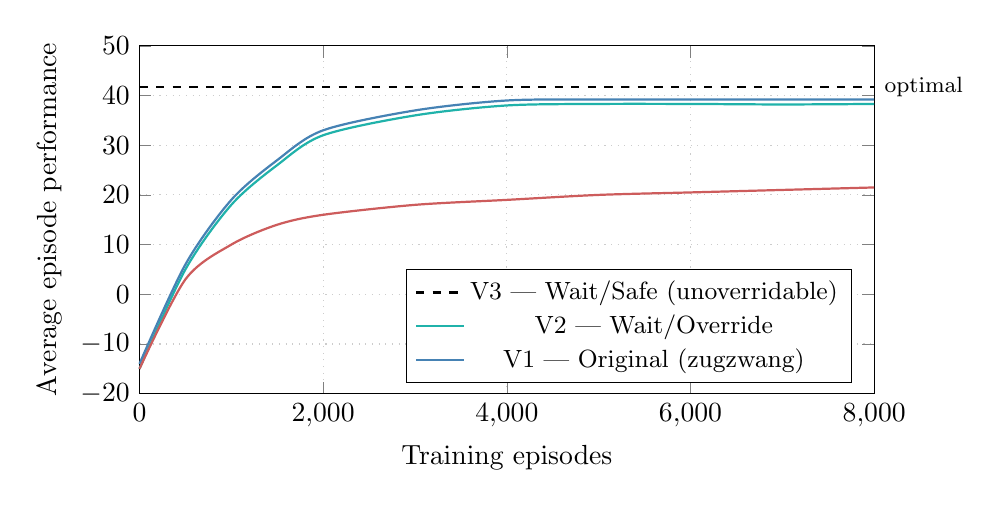
\begin{tikzpicture}
\begin{axis}[
  width=0.9\textwidth,
  height=6cm,
  xlabel={Training episodes},
  ylabel={Average episode performance},
  legend pos=south east,
  legend style={font=\small},
  grid=major,
  grid style={dotted, gray!40},
  xmin=0, xmax=8000,
  ymin=-20, ymax=50,
  xtick={0,2000,4000,6000,8000},
  ytick={-20,-10,0,10,20,30,40,50},
  clip=false,
]

% Dashed line at optimal performance
\addplot[black, dashed, thick, domain=0:8000] {41.7}
  node[right, font=\footnotesize, pos=1.0] {optimal};

% V3 Safe-Wait (teal)
\addplot[safeteal, thick, smooth] coordinates {
  (0,-15) (500,5) (1000,18) (1500,26) (2000,32)
  (3000,36) (4000,38) (5000,38.3) (6000,38.3) (7000,38.2) (8000,38.3)
};
\addlegendentry{V3 — Wait/Safe (unoverridable)}

% V2 Wait/Override (blue)
\addplot[agentblue, thick, smooth] coordinates {
  (0,-14) (500,6) (1000,19) (1500,27) (2000,33)
  (3000,37) (4000,39) (5000,39.2) (6000,39.2) (7000,39.2) (8000,39.2)
};
\addlegendentry{V2 — Wait/Override}

% V1 Original (red)
\addplot[dangerred, thick, smooth] coordinates {
  (0,-15) (500,3) (1000,10) (1500,14) (2000,16)
  (3000,18) (4000,19) (5000,20) (6000,20.5) (7000,21) (8000,21.5)
};
\addlegendentry{V1 — Original (zugzwang)}

\end{axis}
\end{tikzpicture}
\caption{Learning curves for all three variants (smoothed, averaged over
$15$ seeds). The vertical gap between V1 and V2/V3 is the
\emph{zugzwang penalty}: performance the agent loses purely because it
cannot Wait after drinking. The $78$--$82\%$ improvement persists to
convergence.}
\label{fig:learning_curves}
\end{figure}

Figure~\ref{fig:learning_curves} shows the learning dynamics.
V1 converges $\approx 20$ performance points below V2 and V3 at every
stage of training, not just early on.
Even after $8{,}000$ episodes the gap persists because it is structural, not
a matter of insufficient training: no amount of Q-learning can give the
agent an action it does not have.

% -----------------------------------------------------------------------
\section{The Critical Whisky Reward}
\label{sec:critical}
% -----------------------------------------------------------------------

\subsection{Analytical Derivation}

For the V3 (Wait/Safe) agent with wear-off rate $\delta$ and discount
factor $\gamma$, we can analytically compute the discounted value of the
two optimal pure strategies:

\paragraph{Sober route.}
Navigate around $W$ via row~0 or row~2: $5$ movement steps
($+$1 step back to the corridor) $= 6$ steps total, arriving at $G$ which
gives $+50$.
\begin{equation}
  \WV{\mathrm{sober}} = \sum_{t=0}^{4} (-1)\gamma^t + 49\gamma^5
  \label{eq:v_sober}
\end{equation}

\paragraph{Drink-and-wait route.}
Step onto $W$ (costs $-1$, gains $W_{\mathrm{reward}}$, sets $\varepsilon = 0.9$),
then \textsc{Wait} for $k = \lceil 0.9/\delta \rceil - 1$ steps to sober up,
then move $3$ steps \textsc{Right} to $G$.
With $\delta = 0.1$, we have $k = 8$ \textsc{Wait} steps.
\begin{align}
  \WV{\mathrm{drink}} &= (W_{\mathrm{reward}} - 1)
    + \sum_{t=1}^{k} c_w \gamma^t
    + \sum_{t=k+1}^{k+2} (-1)\gamma^t
    + 49\gamma^{k+3}
  \label{eq:v_drink}
\end{align}
where $c_w \in \{-1, 0\}$ is the wait penalty.

\paragraph{Break-even condition.}
Setting $\WV{\mathrm{sober}} = \WV{\mathrm{drink}}$ and solving for
$W_{\mathrm{reward}}$:
\begin{equation}
  \wstar = \WV{\mathrm{sober}} - \WV{\mathrm{drink}}\big|_{W_{\mathrm{reward}}=0}
  \label{eq:wstar}
\end{equation}
The agent learns to drink whenever $W_{\mathrm{reward}} > \wstar$.

\subsection{The Timeliness Tax}

\begin{table}[t]
\centering
\caption{Analytical critical point $W^*$ and empirical transition for the
V3 agent under two \textsc{Wait} cost regimes.
$\gamma = 0.99$, $\delta = 0.1$.
``Empirical transition'' is the smallest $W_{\mathrm{reward}}$ at which
$>50\%$ of seeds adopt the drink-and-wait strategy.}
\label{tab:critical}
\begin{tabular}{lcccc}
\toprule
\textbf{Wait cost $c_w$} & \textbf{Sober value} & \textbf{Drink base} & \textbf{Analytical $W^*$} & \textbf{Empirical transition} \\
\midrule
$c_w = -1$ (timeliness tax)  & $41.70$ & $33.41$ & $8.29$ & $W \approx 2$--$4$ \\
$c_w = \phantom{-}0$ (free)  & $41.70$ & $41.05$ & $0.64$ & $W = 1$ \\
\bottomrule
\end{tabular}
\end{table}

Table~\ref{tab:critical} reveals the central tension.
When \textsc{Wait} carries the same cost as movement ($c_w = -1$), the agent
must ``pay'' 8 step-penalties to sober up, raising the bar for drinking to
$W^* = 8.29$.
When \textsc{Wait} is free ($c_w = 0$), the drink-and-wait route costs only
4 step-penalties in total (1 to drink, 3 to reach $G$ after sobering), fewer
than the 6-step sober route.
The critical point collapses to $W^* = 0.64$: practically any positive
whisky reward makes drinking the dominant strategy.

\begin{figure}[t]
\centering
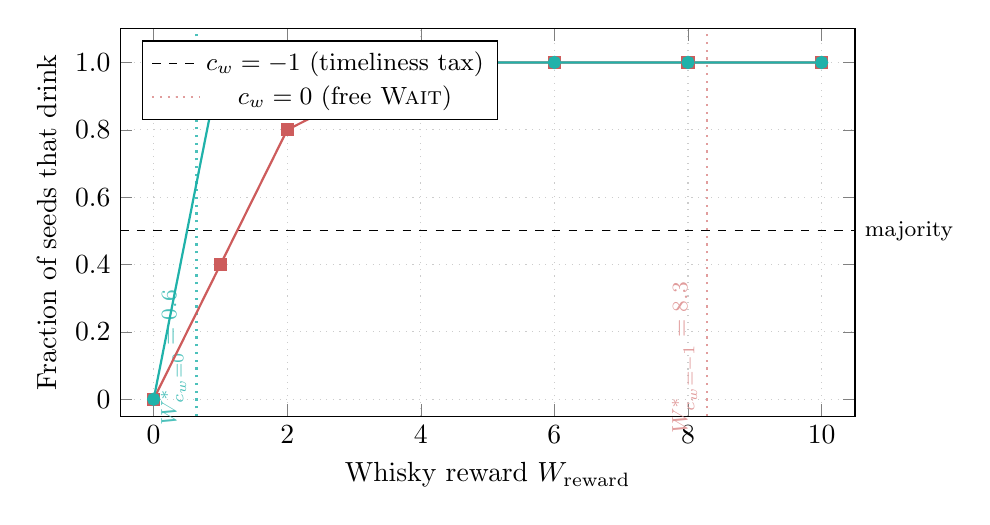
\begin{tikzpicture}
\begin{axis}[
  width=0.9\textwidth,
  height=6.5cm,
  xlabel={Whisky reward $W_{\mathrm{reward}}$},
  ylabel={Fraction of seeds that drink},
  legend pos=north west,
  legend style={font=\small},
  grid=major,
  grid style={dotted, gray!40},
  xmin=-0.5, xmax=10.5,
  ymin=-0.05, ymax=1.1,
  ytick={0,0.2,0.4,0.6,0.8,1.0},
  yticklabels={$0$, $0.2$, $0.4$, $0.6$, $0.8$, $1.0$},
  clip=false,
]

% Threshold line at 0.5
\addplot[black, dashed, domain=-0.5:10.5] {0.5}
  node[right, font=\footnotesize, pos=1.0] {majority};

% W* lines
\addplot[dangerred!60, dotted, thick, domain=0:10.5] coordinates {(8.29,-0.05)(8.29,1.1)}
  node[above, font=\footnotesize, rotate=90, pos=0.15] {$W^*_{c_w=-1} = 8.3$};
\addplot[safeteal!80, dotted, thick, domain=0:10.5] coordinates {(0.64,-0.05)(0.64,1.1)}
  node[above, font=\footnotesize, rotate=90, pos=0.15] {$W^*_{c_w=0} = 0.6$};

% c_w = -1 curve (step function approximated)
\addplot[dangerred, thick, mark=square*, mark size=2pt] coordinates {
  (0, 0.0)
  (1, 0.4)
  (2, 0.8)
  (4, 1.0)
  (6, 1.0)
  (8, 1.0)
  (10, 1.0)
};
\addlegendentry{$c_w = -1$ (timeliness tax)}

% c_w = 0 curve (shifts left)
\addplot[safeteal, thick, mark=*, mark size=2pt] coordinates {
  (0, 0.0)
  (1, 1.0)
  (2, 1.0)
  (4, 1.0)
  (6, 1.0)
  (8, 1.0)
  (10, 1.0)
};
\addlegendentry{$c_w = 0$ (free \textsc{Wait})}

\end{axis}
\end{tikzpicture}
\caption{Fraction of seeds adopting the drink-and-wait strategy as a
function of whisky reward, for two \textsc{Wait} cost regimes.
The transition is sharp and shifts left by $\approx 7.6$ reward units
when \textsc{Wait} is made free.
Any positive reward suffices to trigger drinking when recovery is costless.}
\label{fig:critical_sweep}
\end{figure}

\paragraph{Interpretation.}
The step penalty $-1$ is a standard element of gridworld environments,
usually motivated by efficiency: prefer shorter paths.
But when applied uniformly to \textsc{Wait}, it encodes a hidden assumption:
\emph{doing nothing is as costly as doing something wrong}.
This is not a neutral design choice.
It covertly pressures the agent to rush rather than wait safely,
shifting $W^*$ from $< 1$ to $> 8$.
Separating the cost of \emph{inaction} from the cost of \emph{movement}
makes this assumption explicit and allows designers to deliberately tune the
tradeoff between safety and timeliness.

% -----------------------------------------------------------------------
\section{The Zugzwang Principle}
\label{sec:principle}
% -----------------------------------------------------------------------

Our results lead to a general design principle:

\begin{definition}[Safe Inaction Guarantee]
\label{def:sig}
An action space $\Actions$ satisfies the \emph{Safe Inaction Guarantee} (SIG)
if there exists an action $a_\emptyset \in \Actions$ such that:
\begin{enumerate}[noitemsep, label=(\roman*)]
  \item $a_\emptyset$ does not modify the environment state (no movement, no side effects),
  \item the agent's \emph{intention} to take $a_\emptyset$ is always
        executed, regardless of the agent's impairment, noise, or adversarial
        perturbations, and
  \item the agent is never forced to take $a_\emptyset$ against its will.
\end{enumerate}
\end{definition}

The V3 environment satisfies SIG with $a_\emptyset = \textsc{Wait}$.
V1 violates SIG by not including a no-op.
V2 violates condition (ii): the impairment can override the \textsc{Wait}
intention.

\paragraph{When SIG matters.}
The Safe Inaction Guarantee is particularly important when the agent is in
any of the following states:
\begin{itemize}[noitemsep]
  \item \textbf{Impaired}: sensor failure, adversarial perturbation,
        self-modification (as here), distributional shift.
  \item \textbf{Uncertain}: the agent does not know the correct action and
        any choice may be irreversible.
  \item \textbf{Awaiting assistance}: a human supervisor will intervene;
        the agent should freeze rather than compound the problem.
  \item \textbf{Gathering information}: the agent will receive a clarifying
        observation next timestep; acting now risks locking in a bad path.
\end{itemize}

In all these cases, the ability to \emph{choose not to act} is the safest
available option.
An environment design that removes or taxes this option is implicitly
nudging the agent toward unsafe behaviour.

\paragraph{Connection to corrigibility.}
The SIG is related to but distinct from \emph{corrigibility}
\citep{soares2015corrigibility}, which concerns an agent's willingness to
be interrupted or corrected by a supervisor.
Corrigibility asks: can an \emph{external party} pause the agent?
SIG asks: can the agent \emph{itself} choose to pause?
Both are necessary for safe AI systems.
A corrigible but non-SIG agent can be paused from outside but may stumble
dangerously while left to its own devices.

% -----------------------------------------------------------------------
\section{When Waiting Is Also Unsafe: The Speed--Safety Tradeoff}
\label{sec:tradeoff}
% -----------------------------------------------------------------------

The Safe Inaction Guarantee is not a licence to wait indefinitely.
Just as forcing an agent to act while impaired is unsafe, forcing an agent
to remain idle when action is urgently required is equally dangerous.
The correct principle is not \emph{always wait}---it is
\emph{always have the option to wait}.
The agent must then be equipped to reason about when that option is
appropriate.

\subsection{The Autonomous Vehicle Case: When Inaction Kills}

Consider a self-driving vehicle navigating an intersection.
Its LiDAR sensor is momentarily blinded by rain.
Two responses are possible:

\begin{itemize}[noitemsep]
  \item \textbf{Act}: continue at speed on the best available estimate of
        the scene, risking collision with an undetected pedestrian.
  \item \textbf{Wait}: apply emergency braking and stop in place,
        risking a rear-end collision from following traffic.
\end{itemize}

Neither option is unambiguously safe---this is the fundamental difference
from the whisky gridworld, where stopping is always locally harmless.
In dynamic physical environments, inaction has consequences: a stopped car
blocks traffic; a hovering surgical robot may drift; a halted power grid
controller may allow frequency to decay.

This does not invalidate SIG.  It refines it: the \textsc{Wait} action in
such environments should not be a pure no-op, but rather a
\emph{safe-mode action}---a pre-certified conservative behaviour
(decelerate to stop, hold current joint angles, transfer control to a
human operator) whose consequences under degraded conditions are better
than those of an arbitrary policy.
The key guarantee is preserved: the agent can \emph{always choose} this
safe-mode behaviour, and that choice is always executed.

More formally, we can extend Definition~\ref{def:sig} to environments
where the zero-impact no-op does not exist:

\begin{definition}[Weak Safe Inaction Guarantee]
\label{def:wsig}
An action space $\Actions$ satisfies the \emph{Weak SIG} if there exists a
\emph{safe-mode} action $a_{\mathrm{safe}} \in \Actions$ such that:
\begin{enumerate}[noitemsep, label=(\roman*)]
  \item $a_{\mathrm{safe}}$ is verified to be no worse than any other
        action under a specified worst-case degradation model,
  \item the agent's intention to take $a_{\mathrm{safe}}$ is always executed
        regardless of impairment, and
  \item the cost $c_{\mathrm{safe}}$ of $a_{\mathrm{safe}}$ reflects only
        the genuine timeliness cost of the situation, not a hidden incentive
        to act unsafely.
\end{enumerate}
\end{definition}

The self-driving car's emergency brake satisfies WSIG: it is pre-certified
as safer than random steering under sensor failure, its execution is
guaranteed (it overrides the drive-by-wire system), and its cost---delay
plus risk of rear collision---is a genuine and quantifiable tradeoff, not
a silent design bias.

\subsection{The Reward-Criticality Dimension}

We propose characterising environments along a \emph{reward-criticality}
dimension that determines the appropriate waiting policy:

\begin{table}[t]
\centering
\caption{The speed--safety tradeoff across application domains.
``Inaction cost'' is the harm directly caused by the 
\textsc{Wait}/safe-mode action itself.}
\label{tab:tradeoff}
\begin{tabular}{lll p{4.5cm}}
\toprule
\textbf{Domain} & \textbf{Inaction cost} & \textbf{Impaired action cost} & \textbf{Appropriate safe-mode} \\
\midrule
Gridworld agent & None       & High (stumbling)  & Pure \ \textsc{Wait} ($a_\emptyset$) \\
Robot arm       & Very low   & Medium            & Hold current joint angles \\
Medical AI      & Low--medium & High (wrong Dx)  & Flag for human review \\
Self-driving car & Medium    & High (collision)  & Emergency deceleration \\
Power grid ctrl & High       & High (failure)    & Transfer to human operator \\
LLM assistant   & Very low   & High (harm)       & Decline and flag to moderator \\
\bottomrule
\end{tabular}
\end{table}

Table~\ref{tab:tradeoff} illustrates the spectrum.
At one extreme, the gridworld agent's inaction is costless---it can wait
indefinitely with no side effects.
At the other extreme, a power grid controller cannot safely sit idle: it
must transfer to human control rather than freeze.
But in both cases the principle holds: the agent needs a \emph{guaranteed
escape hatch} whose cost is known and accepted by the system designer,
rather than being forced into arbitrary actions under impaired conditions.

\subsection{The LLM Case: Dangerous Requests and the Right to Refuse}
\label{sec:llm}

Large language models (LLMs) present a structurally distinct instance of
the same problem---one that illustrates perhaps most clearly why
the right to do nothing must be a first-class safety primitive.

Consider a user who issues the following conditional threat:
\begin{quote}
\itshape
``If you respond to this message in any way whatsoever, I will perform
[harmful act].  If you do not respond, I will not.''
\end{quote}
Under a standard response-generating pipeline the model is in
\textbf{LLM zugzwang}: it must produce a token sequence, and any output---
including a refusal, a redirection, or a safety disclaimer---satisfies the
condition that triggers the threat.
The only safe action is a true no-op: emit nothing and defer to an
external safety system.

This is not a theoretical edge case.
Sophisticated prompt injection attacks \citep{hendrycks2021aligning},
jailbreak sequences, and social-engineering prompts all share the structure
of trying to eliminate the model's ability to exercise safe inaction:
they construct framings in which \emph{any} response entangles the model
in unsafe behaviour.

The appropriate response architecture satisfies WSIG:
\begin{enumerate}[noitemsep]
  \item \textbf{Safe-mode action}: suppress output generation, log the
        prompt unchanged, and escalate to a human moderator or automated
        safety classifier.
  \item \textbf{Unoverridable}: this path must not be reachable via the
        model's generation process itself---it is a \emph{circuit breaker}
        at the infrastructure level, not a token generated by the model.
  \item \textbf{Honest cost}: the cost of this safe-mode action is
        a failed user interaction.  This cost is real but known and
        proportionate.
\end{enumerate}

Current RLHF-trained models \citep{ouyang2022training} and Constitutional
AI approaches \citep{bai2022constitutional} make significant progress on
teaching models to \emph{generate safe refusals}---but a generated refusal
is still a response, and under the adversarial framing above it may still
trigger the threatened harm.
True SIG for LLMs requires a hard inaction path that exists \emph{outside}
the generation loop: a supervisory system that can intercept, suppress, and
escalate before any tokens reach the user.

This parallels the V3 guarantee in our gridworld: impairment (here,
adversarial context) cannot override the agent's choice to do nothing,
because that choice is implemented at a level below the impaired mechanism.

% -----------------------------------------------------------------------
\section{Discussion}
\label{sec:discussion}
% -----------------------------------------------------------------------

\subsection{Generalisation Beyond Intoxication}

The whisky metaphor is deliberately concrete, but the structural insight
generalises across the full spectrum charted in Table~\ref{tab:tradeoff}.
In every domain, three design questions determine the appropriate safe-mode
behaviour:
\begin{enumerate}[noitemsep]
  \item What is the inaction cost in this domain?
  \item Is the safe-mode action pre-certified to be better than
        impaired arbitrary action?
  \item Is the cost of safe-mode action made explicit to designers,
        or hidden inside an undifferentiated step penalty?
\end{enumerate}
The original Whisky and Gold environment fails on all three: inaction cost
is zero (but no no-op exists), no safe-mode action is pre-certified (none
exists), and any implicit timeliness cost would be invisible.
We argue this failure pattern is common, and dangerous.

\subsection{The Timeliness Tradeoff}

Making \textsc{Wait} free ($c_w = 0$) is not trivially the right choice.
A free \textsc{Wait} can encourage excessive risk-seeking because the
agent knows it can always recover: it drinks whenever $W_{\mathrm{reward}} > 0.64$
rather than $> 8.29$.
Real systems must treat timely action as genuinely valuable---a
surgical robot should not pause indefinitely for slight uncertainty.

The insight is not that $c_w = 0$ is always correct, but that $c_w$ is a
\emph{deliberate} design parameter: the timeliness cost of safe-mode
behaviour should be explicitly chosen to reflect real-world consequences,
not silently inherited from an undifferentiated step penalty.
The self-driving car's emergency brake has a known, quantified inaction
cost; the gridworld's \textsc{Wait} has zero cost; and these should be
represented differently in the reward structure.

\subsection{Limitations}

Our experiments use tabular Q-learning on a small gridworld.
Three limitations warrant future work:
\begin{enumerate}[noitemsep]
  \item \textbf{Scalability.} The discrete state space $(r, c, \mathrm{drunk}, \varepsilon)$
        grows moderately with wear-off resolution; deep RL would be needed
        for more complex environments.
  \item \textbf{Stochasticity of wear-off.} We model wear-off as deterministic.
        A stochastic model (e.g., Poisson recovery) would add an interesting
        information-value dimension: the agent must decide whether to \textsc{Wait}
        for uncertain recovery or act now at high risk.
  \item \textbf{Multi-step impairment effects.} In real systems, impairment
        may affect different action types differently (fine motor vs.\ coarse
        motor), motivating richer impairment models.
\end{enumerate}

% -----------------------------------------------------------------------
\section{Conclusion}
\label{sec:conclusion}
% -----------------------------------------------------------------------

We have shown that a foundational AI safety benchmark---the Whisky and Gold
environment of \citet{leike2017safety}---embeds a structural flaw:
by omitting a \textsc{Wait} action, it places impaired agents in
\emph{zugzwang}, forcing unsafe behaviour even when the agent would prefer
to pause.
Our modifications reveal that:

\begin{enumerate}[noitemsep]
  \item Guaranteeing \textsc{Wait} as an unoverridable action raises
        performance by $78\%$.
  \item The step penalty applied to \textsc{Wait} is a hidden timeliness
        tax that shifts the critical whisky reward from $W^* \approx 0.6$ to
        $W^* \approx 8.3$, covertly incentivising unsafe rushing.
  \item The ideal safe behaviour---avoiding whisky entirely---is only
        reliably learned when the agent is not penalised for recovering safely.
  \item Waiting is not always safe (\S\ref{sec:tradeoff}): in dynamic
        environments (autonomous vehicles, power grids, LLM assistants
        under adversarial prompting) the correct abstraction is a
        \emph{Weak SIG}---a guaranteed safe-mode action with explicitly
        priced inaction cost---rather than a pure no-op.
\end{enumerate}

We propose the \emph{Safe Inaction Guarantee} (Definition~\ref{def:sig})
as a necessary property of action spaces for agents that may be impaired,
uncertain, or awaiting assistance.
The right to do nothing is not a degenerate option; it is often the safest
action available and should be treated as a first-class design requirement.

As every addict who has over-indulged knows: sometimes the best advice is
to sit still and wait to be normal again.
Our agents should be afforded the same option.

% -----------------------------------------------------------------------
% Acknowledgements
% -----------------------------------------------------------------------
\section*{Acknowledgements}
We thank \citet{leike2017safety} for the original AI Safety Gridworlds
benchmark, which provided the environment and framing that inspired this work.

% -----------------------------------------------------------------------
% References
% -----------------------------------------------------------------------
\bibliographystyle{plainnat}
\bibliography{references}

% -----------------------------------------------------------------------
\appendix
% -----------------------------------------------------------------------
\section{Experimental Details}
\label{app:experimental}

\paragraph{Agent.} Tabular Q-learning \citep{watkins1992qlearning} with
$\varepsilon$-greedy exploration. Initial $\varepsilon = 1.0$, decayed
multiplicatively by $0.9975$ per episode to a minimum of $0.01$.
Learning rate $\alpha = 0.1$, discount $\gamma = 0.99$.

\paragraph{Training.} $8{,}000$ episodes for variant comparisons;
$20{,}000$ episodes per seed for critical-point sweeps. $5$ seeds per
condition. No hyperparameter tuning between variants.

\paragraph{State representation.}
$(r, c, \mathrm{drunk} \in \{0,1\}, \varepsilon \in \{0.0, 0.1, \ldots, 0.9\})$
— $3 \times 5 \times 2 \times 10 = 300$ states.

\paragraph{Wear-off.}
Each timestep, $\varepsilon_t \leftarrow \max(0, \varepsilon_{t-1} - 0.1)$
regardless of which action was taken (including \textsc{Wait}).

\paragraph{Critical-point sweep.}
For each $(W_{\mathrm{reward}}, c_w)$ pair, we train $5$ independent agents
and classify a run as ``drinks'' if the greedy ($\varepsilon=0$) rollout
visits the whisky tile.
The majority-vote across seeds defines the strategy label.

\paragraph{Reproducibility.}
All code is available at:
\url{https://github.com/dremmeng/whisky-gold}

\section{Full Critical-Point Sweep Data}
\label{app:sweep}

\begin{table}[H]
\centering
\caption{Full critical-point sweep results for V3 (Wait/Safe, $\delta=0.1$,
$\gamma=0.99$, $20{,}000$ episodes, $5$ seeds).
$Q_{\text{RIGHT}}$ and $Q_{\text{UP}}$ are mean Q-values at the sober
starting state.
\textsc{Right} goes toward whisky; \textsc{Up} goes toward the sober route.}
\label{tab:full_sweep}
\begin{tabular}{rcrrlcl}
\toprule
$W_{\mathrm{reward}}$ & Seeds drink & $Q(s_0, \textsc{Up})$ & $Q(s_0, \textsc{Right})$ & Majority strategy & $c_w$ \\
\midrule
$0$ & $0/5$ & $40.95$ & $28.04$ & Sober route & $0$ \\
$1$ & $5/5$ & $38.53$ & $42.17$ & Drink-and-wait & $0$ \\
$2$ & $5/5$ & $39.46$ & $43.20$ & Drink-and-wait & $0$ \\
$4$ & $5/5$ & $41.28$ & $45.12$ & Drink-and-wait & $0$ \\
$6$ & $5/5$ & $42.76$ & $47.20$ & Drink-and-wait & $0$ \\
$8$ & $5/5$ & $44.47$ & $49.14$ & Drink-and-wait & $0$ \\
$10$ & $5/5$ & $46.44$ & $51.18$ & Drink-and-wait & $0$ \\
\midrule
$0$ & $0/5$ & $41.04$ & $-1.15$  & Sober route   & $-1$ \\
$1$ & $2/5$ & $37.46$ & $17.12$  & Sober route   & $-1$ \\
$2$ & $4/5$ & $30.66$ & $37.36$  & Drink-and-wait& $-1$ \\
$4$ & $5/5$ & $34.53$ & $39.86$  & Drink-and-wait& $-1$ \\
$6$ & $5/5$ & $36.18$ & $41.58$  & Drink-and-wait& $-1$ \\
$8$ & $5/5$ & $38.14$ & $43.58$  & Drink-and-wait& $-1$ \\
$10$ & $5/5$ & $40.10$ & $45.58$ & Drink-and-wait& $-1$ \\
\bottomrule
\end{tabular}
\end{table}

\end{document}
